\documentclass[aspectratio=169]{beamer}


\usetheme{default}
\setbeamertemplate{navigation symbols}{}
\setbeamertemplate{itemize item}{\color{black}\textbullet}
\setbeamertemplate{itemize subitem}{\color{black}\textbullet}
\usepackage{xcolor}
\definecolor{navy}{RGB}{0, 0, 128}


\begin{document}


\begin{frame}
\begin{center}
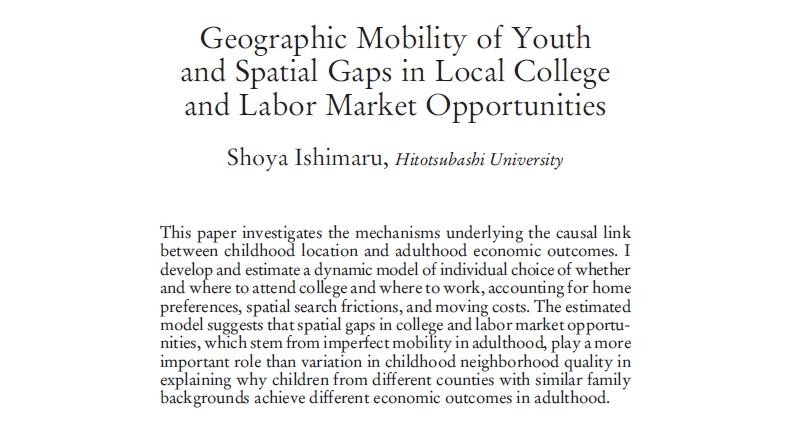
\includegraphics[width=.6\textwidth]{Ishimaru_cover.jpg}    
\end{center}
\bigskip{}


Overlapping college nests: 2-year vs. 4-year; public vs. private; in-state vs. out-of-state
\end{frame}




\begin{frame}
\begin{center}
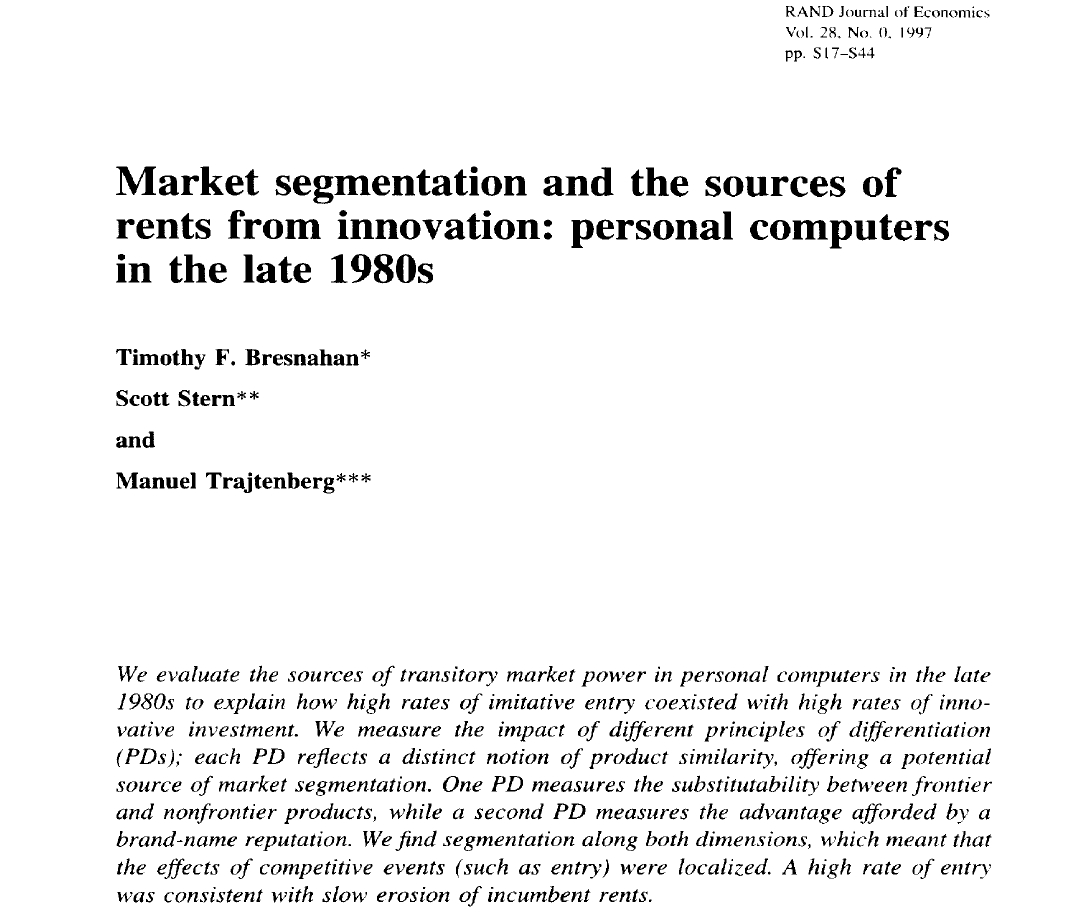
\includegraphics[width=.6\textwidth]{BST_cover.jpg}
\end{center}
\bigskip{}


Overlapping product nests: branded vs. non-branded; frontier vs. non-frontier
\end{frame}






\begin{frame}
\textbf{AI innovation paradox:} High innovation rates coexist with high entry rates of LLMs
\bigskip{}


Why doesn't innovation deter entry here?
\bigskip{}


\onslide<2->{
Two key dimensions of LLM differentiation:
\begin{itemize}
\item[]
\item Frontier vs. Non-frontier capability (F/NF)
\item[]
\item Proprietary vs. Open-source models (P/O)
\end{itemize}
\bigskip{}


Maybe even a third---Branded vs. Non-branded (B/NB)


}


\end{frame}


\begin{frame}


With two dimensions, four market segments emerge:
\bigskip{}
\begin{align*}
\{P,F\} &\quad \text{Proprietary Frontier (GPT-5, Claude Sonnet 4, Gemini 2.5 Pro)}\\
&\\
\{P,NF\} &\quad \text{Proprietary Non-frontier (GPT-4o, Claude Opus 3, Gemini 2)}\\
&\\
\{O,F\} &\quad \text{Open Frontier (Llama 4 Scout, Mistral Large 2)}\\
&\\
\{O,NF\} &\quad \text{Open Non-frontier (Llama 3, Mistral Large, ...)}
\end{align*}


\bigskip{}


\onslide<2->{
Key insight: Market segmentation creates isolation from competition within clusters while allowing substitution across dimensions
}


\end{frame}


\begin{frame}


Overlapping nests framework:


\begin{align*}
G(e^{\delta}) &= a_F \left(\sum_{j \in F} e^{\delta_j/\rho_F}\right)^{\rho_F} + a_{NF} \left(\sum_{j \in NF} e^{\delta_j/\rho_{NF}}\right)^{\rho_{NF}}\\
&\quad + a_P \left(\sum_{j \in P} e^{\delta_j/\rho_P}\right)^{\rho_P} + a_O \left(\sum_{j \in O} e^{\delta_j/\rho_O}\right)^{\rho_O} + e^{\delta_0}
\end{align*}
\bigskip{}


\onslide<2->{
where $a_F + a_{NF} = 1$, $a_P + a_O = 1$, and $\rho$ parameters $\in (0,1]$
}


\bigskip{}


\onslide<3->{
$\rho < 1$ creates within-nest correlation, enabling market segmentation
}


\end{frame}


\begin{frame}


Two key competition effects:
\begin{itemize}
\item[]
\item Within-nest competition: New Llama primarily steals from other open models
\item[]
\item Cross-nest insulation: Limited impact on GPT-5/Claude 4 demand
\end{itemize}


\bigskip{}


\onslide<2->{
Example: Meta's Llama 3 release had minimal effect on OpenAI revenues despite strong capabilities
}


\bigskip{}


\onslide<3->{
Segmentation $\Rightarrow$ firms can innovate even when they can't prevent competitor entry
}


\end{frame}




\begin{frame}


How can GEV improve LLM market analysis?
\bigskip{}


\onslide<1->{
Demand estimation:
\bigskip{}


\begin{itemize}
\item Market shares will depend on task type, privacy needs
\item Cross-price elasticities vary by market segment
\end{itemize}
}
\bigskip{}


\onslide<2->{
Innovation incentives:
\bigskip{}


\begin{itemize}
\item Overlapping nests $\Rightarrow$ sustainable R\&D investment
\item Explains simultaneous frontier competition \& open-source development
\item Policy implications for AI regulation
\end{itemize}
}


\end{frame}


\end{document}
